% !TEX root =  ../main_manuscript.tex 
\section{Personalized Schedule of Invasive Tests for Detecting Progression}
\label{sec:schedule}
We intend to develop a personalized schedule of invasive tests for a new patient $j$, not present in training dataset $\mathcal{A}_n$. Tests are conducted only until progression is detected (Figure~\ref{fig:delay_explanation}). Let $T^*_j$ be the true time of progression, and ${t < T^*_j}$ be the time of the last conducted test on which progression was not detected for the $j$-th patient. Lastly, ${v > t}$ denotes the time of the current follow-up visit.

\subsection{Cumulative-risk of progression}
\label{subsec:cum_risk}
First we combine the history of observed longitudinal outcomes $\{\mathcal{Y}_{1j}(v), \ldots, \mathcal{Y}_{Kj}(v)\}$ until the current visit time $v$, and the result of the last conducted test ${T^*_j > t}$ to define the patient-specific cumulative-risk of progression at future time $u$ (Figure~\ref{fig:dynrisk_explanation}).
\begin{equation}
\label{eq:cumulative_risk}
\begin{split}
R_j(u \mid t, v) &= \mbox{Pr}\big\{T^*_j \leq u \mid T^*_j > t, \mathcal{Y}_{1j}(v), \ldots, \mathcal{Y}_{Kj}(v), \mathcal{A}_n\big\}\\
&=\int \int \mbox{Pr}(T^*_j \leq u \mid T^*_j > t, \boldsymbol{b}_{j}, \boldsymbol{\theta}) p\big\{\boldsymbol{b}_j \mid T^*_j > t, \mathcal{Y}_{1j}(v), \ldots, \mathcal{Y}_{Kj}(v), \boldsymbol{\theta} \big\}\\
&\quad \times p(\boldsymbol{\theta} \mid \mathcal{A}_n) \mathrm{d}\boldsymbol{b}_j \mathrm{d}\boldsymbol{\theta}, \quad u \geq t.
\end{split}
\end{equation}
The personalized cumulative-risk function $R_j(\cdot)$ depends on the observed longitudinal data $\{\mathcal{Y}_{1j}(v), \ldots, \mathcal{Y}_{Kj}(v)\}$, and the training dataset $\mathcal{A}_n$ via the posterior distribution of patient-specific random effects~$\boldsymbol{b}_j$, and posterior distribution of the vector of joint model parameters~$\boldsymbol{\theta}$, respectively. The risk also dynamically updates as more longitudinal data becomes available over follow-up (Panel~B~and~C, Figure~\ref{fig:dynrisk_explanation}).

\begin{figure}
\centerline{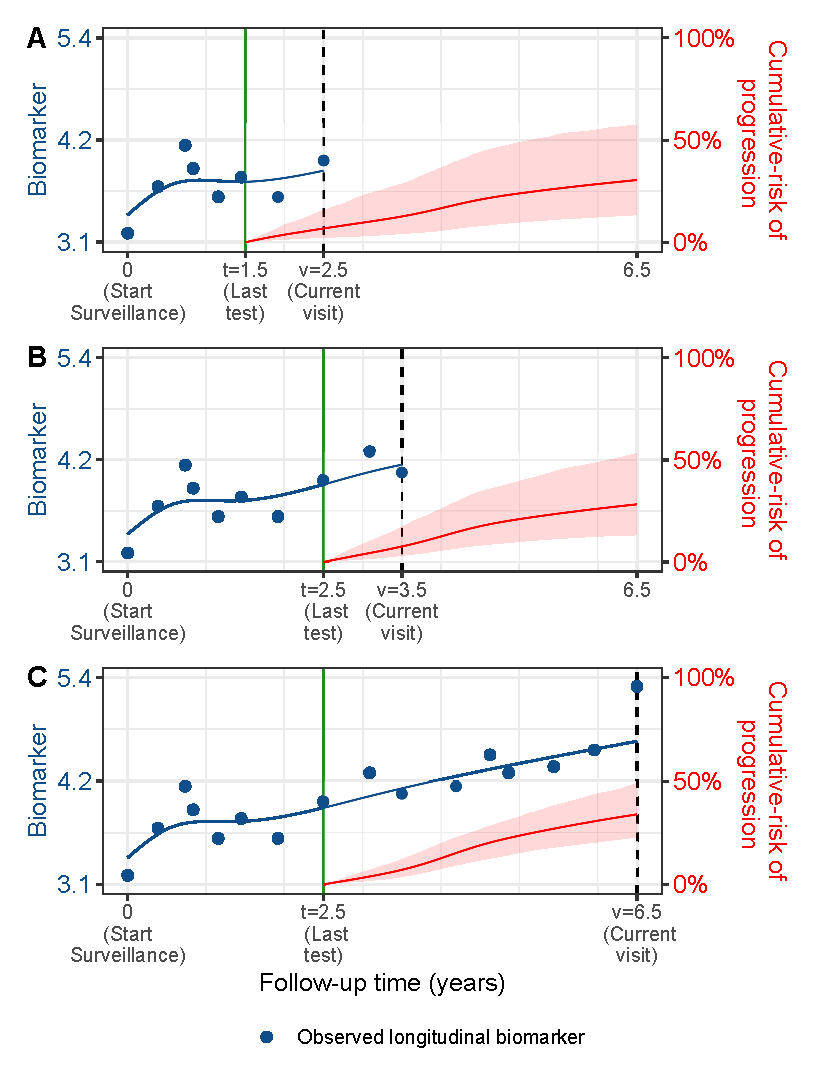
\includegraphics{images/dynrisk_plot_102.eps}}
\caption{\textbf{Cumulative-risk of progression changing dynamically over follow-up} as more patient data is gathered. A single longitudinal outcome, namely, a continuous biomarker of disease progression, is used for illustration. \textbf{Panels~A,~B~and~C:} are ordered by the time of the current visit (dashed vertical black line) of a new patient. At each of these visits, we combine the accumulated longitudinal measurements (shown in blue), and last time of negative invasive test (solid vertical green line) to obtain the updated cumulative-risk profile (shown in red) of the patient. All values are illustrative.} 
\label{fig:dynrisk_explanation}
\end{figure}

\subsection{Personalized Schedule of Tests Using a Cumulative-risk Threshold $\kappa^*$}
\label{subsec:pers_schedule}
Our aim is to employ the cumulative-risk function in~(\ref{eq:cumulative_risk}) to develop a risk-based personalized schedule of invasive tests for the $j$-th patient. Typically an invasive test is decided on the same visit on which auxiliary data (e.g., biomarkers) is measured. Let $U={u_1, \ldots, u_L}$ represent a schedule of such visits (e.g., every six months in prostate cancer for PSA measurement), where $u_1=v$ is also the time of the current visit.

First, we make $L$ successive decisions for conducting tests on each of the $L$ future visit times $u_l \in U$. Specifically, we decide to conduct a test at time $u_l$ if the conditional cumulative-risk of progression at $u_l$ is larger than a certain risk threshold $0 \leq \kappa^* \leq 1$ (e.g., $\kappa^*=10$\% risk). If a test gets planned at time $u_l$, then the successive test decision at time $u_{l+1}$ is made using an updated cumulative-risk profile (Figure~\ref{fig:schedule_explanation}). This updated cumulative-risk profile accounts for the possibility that progression may occur after time $u_l < T^*_j$. The test decisions on each future visit time $u_l$ are defined as: 
\begin{equation*}
\label{eq:personalized_decision_grid}
\begin{split}
Q_j^{\kappa^*}(u_l \mid t_l, v) &= I\big\{R_j(u_l \mid t_l, v) \geq \kappa^* \big\},\\
t_l &= \left\{\begin{array}{lcr}
  t, &\mbox{if}& l=1\\
  t_{l-1}, &\mbox{if}&  Q_j^{\kappa^*}(u_{l-1} \mid t_{l-1}, v)=0, l\geq 2\\ 
  u_{l-1}, &\mbox{if}&  Q_j^{\kappa^*}(u_{l-1} \mid t_{l-1}, v)=1, l\geq 2\\
\end{array} \right\}.
\end{split}
\end{equation*}
The cumulative-risk $R_j(u_l \mid t_l, v)$ at future visit time $u_l$ utilizes the time $t_l$ as the time of the last conducted test on which progression may not be observed (Equation~\ref{eq:cumulative_risk}). However, the contribution of the observed longitudinal data $\{\mathcal{Y}_{1j}(v), \ldots, \mathcal{Y}_{Kj}(v)\}$ in the risk function remains the same over all time points in $U$. The test decision at time $u_l$ is denoted by ${Q_j^{\kappa^*}(u_l \mid t_l, v)}$. Via the indicator function $I(\cdot)$ it obtains a value 1 (or 0) when a test is to be conducted (or not conducted) at time $u_l$. The subset of future time points in $U$ on which a test is to be performed results into a personalized schedule of planned future tests, given by:
\begin{equation}
\label{eq:personalized_schedule_grid}
S_j^{\kappa^*}(U \mid t, v) = \big\{ u_l \in U \mid Q_j^{\kappa^*}(u_l \mid t_l, v)=1\big\}.
\end{equation}
The personalized schedule in~(\ref{eq:personalized_schedule_grid}) is updated as more patient data becomes available over subsequent follow-up visits.

\begin{figure}
\centerline{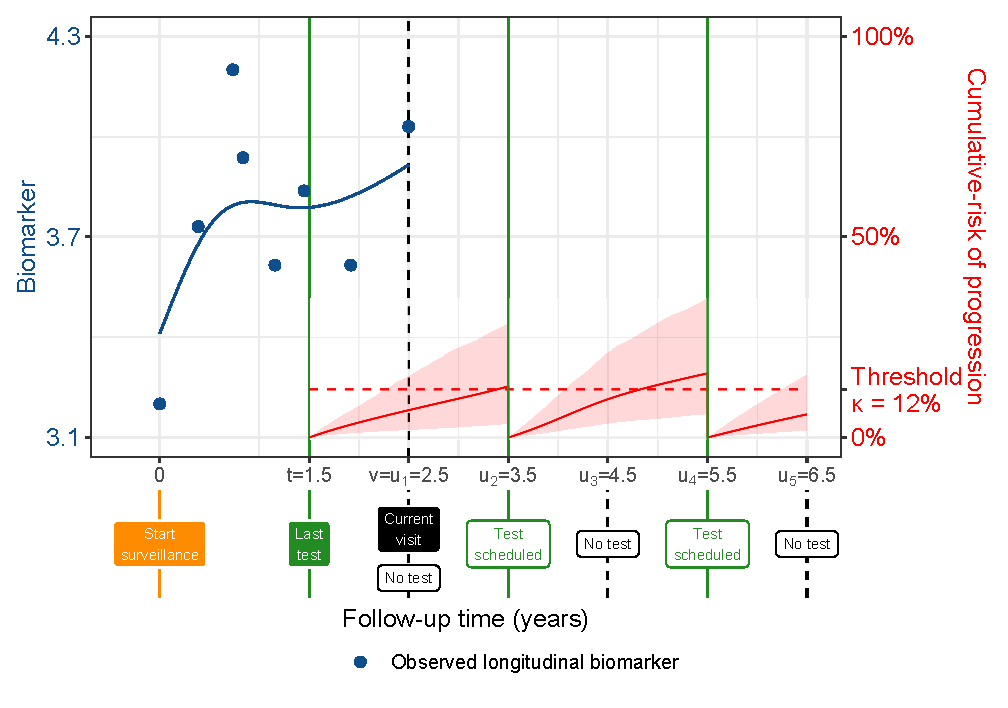
\includegraphics{images/schedule_explanation_102.eps}}
\caption{\textbf{Personalized Invasive Test Schedule Using Patient-specific Conditional Cumulative-risk of Progression}.  A single longitudinal outcome, namely, a continuous biomarker (observed: blue dots, fitted: blue line) of disease progression is used for illustration. The last test on which progression was not observed was conducted at $t=1.5$ years. The current visit time of the patient is $v=2.5$ years. Decisions for invasive test need to be made at a gap of every one year starting from the current visit until a horizon of 6.5 years. That is, $U=\{2.5, 3.5, 4.5, 5.5, 6.5\}$ years. Based on an example risk threshold of 12\% ($\kappa^*=0.12$) the future test decisions at time points in $U$ lead to a personalized schedule $S_j^{\kappa^*} (U \mid t=1.5, v=2.5) = \{3.5, 5.5\}$ years. The conditional cumulative-risk profiles $R_j(u_l \mid t_l, v)$ employed in~(\ref{eq:personalized_decision_grid}) are shown with red line (confidence interval shaded). It is called `conditional' because, for example, the second test at future time 5.5 years, is scheduled after accounting for the possibility that progression (true time $T^*_j$) may not have occurred until the time of the previously scheduled test at time $3.5 < T^*_j$ years. All values are illustrative.} 
\label{fig:schedule_explanation}
\end{figure}

\subsection{Expected Number of Tests and Time Delay in Detecting Progression}
\label{subsec:exp_delay_estimation}
The schedule $S_j^{\kappa^*}(U \mid t, v)$ manifests a personalized test plan for the $j$-the patient. However, the number of tests that will get conducted and the time delay in detecting progression that may subsequently be observed (Figure~\ref{fig:delay_explanation}), depends on the true time of progression $T^*_j$ of the patient. Since two different patients with the same timing of tests will expect different number of tests and time delay, we estimate these two quantities in a patient-specific manner as well. Although, this calculation is not limited to personalized schedules only, but can be done for any schedule $S$ of tests with $N$ time points $S=\{s_n \mid n=1,\ldots, N\}$. 

For each of the $N$ planned tests there exist $N$ time intervals ${s_{n-1} < T^*_j \leq s_n}$ in which progression may be observed. Correspondingly, there are $N$ possible number of tests $1,\ldots, N$, and $N$ possible time delays in detecting progression $s_n - T^*_j$. Given a schedule $S$, the true number of tests $N_j$ and true time delay in detecting progression $D_j$ that the patient will experience can be defined as:
\begin{equation}
\label{eq:number_of_tests_and_delay}
\begin{split}
N_j (S \mid t) &= \left\{ \begin{array}{lcr}
  1, &\mbox{if}& t < T^*_j \leq s_1\\
  \ldots \\
  N-1, &\mbox{if}& s_{N-2} < T^*_j \leq s_{N-1}\\
  N, &\mbox{if}& s_{N-1} < T^*_j  
\end{array} \right\},\\
D_j (S \mid t) &= \left\{ \begin{array}{lcrr}
  s_1 - T^*_j, &\mbox{if}& t < T^*_j \leq s_1\\
  \ldots \\
  s_N - T^*_j, &\mbox{if}& s_{N-1} < T^*_j \leq s_N  
\end{array} \right\}.
\end{split}
\end{equation}
The time delay is not defined for the scenario in which the patient obtains progression after the time of the last test in the schedule $T^*_j > s_N$. To estimate the expected values of both $N_j(\cdot)$ and $D_j(\cdot)$ in a patient-specific manner, we exploit the personalized cumulative-risk profile of the patient (Equation~\ref{eq:cumulative_risk}). Specifically, the expected number of tests $E\{N_j(\cdot)\}$ and expected time delay $E\{D_j(\cdot)\}$ can be calculated as the weighted sum of $N$ possible number of tests and time delays defined in~(\ref{eq:number_of_tests_and_delay}). The $n$-th weight is equal to the probability of the patient obtaining progression in the $n$-th interval ${s_{n-1} < T^*_j \leq s_n}$.
\begin{equation}
\label{eq:expected_number_of_tests_and_delay}
\begin{split}
E\big\{N_j(S \mid t)\big\} &= \sum_{n=1}^{N-1} n \times \mbox{Pr}(s_{n-1} < T^*_j \leq s_n) + N \times \mbox{Pr}(T^*_j > s_{N-1}), \quad s_0 = t\\
E\big\{D_j(S \mid t)\big\} &= \sum_{n=1}^{N} \Big\{s_n - E(T^*_j \mid s_{n-1}, s_n, v)\Big\} \times \mbox{Pr}(s_{n-1} < T^*_j \leq s_n) , \quad s_0 = t\\
E(T^*_j \mid s_{n-1}, s_n, v) &= s_{n-1} + \int_{s_{n-1}}^{s_n} \mbox{Pr}\Big\{T^*_j \geq u \mid s_{n-1} < T^*_j \leq s_n, \mathcal{Y}_{1j}(v), \ldots, \mathcal{Y}_{Kj}(v), \mathcal{A}_n\Big\} \mathrm{d}u\\
\mbox{Pr}(s_{n-1} < T^*_j \leq s_n) &= R_j(s_n \mid t, v) - R_j(s_{n-1} \mid t, v)\\
\mbox{Pr}(T^*_j > s_{N-1}) &= 1- R_j(s_{N-1} \mid t, v),
\end{split}
\end{equation}
where $E(T^*_j \mid s_{n-1}, s_n, v)$ denotes the conditional expected time of progression for the scenario $s_{n-1} < T^*_j \leq s_n$, and is calculated as the area under the corresponding survival curve.

The personalized expected number of tests and expected time delay in detecting progression have the advantage that they are updated over follow-up as more patient data becomes available. Since they can be calculated for any schedule, patients and doctors can utilize them to compare schedules before making a decision. Although, in order to have a fair comparison of time delays between different schedules for the same patient, a compulsory test at a common horizon time point should be planned in all schedules.

\subsection{Choice of Risk Threshold $\kappa^*$}
The risk threshold $\kappa^*$ controls the timing and the total number of invasive tests in the personalized schedule $S_j^{\kappa^*}(U \mid t, v)$. Through the timing and the total number of planned tests, $\kappa^*$ also indirectly affects the time delay (Figure~\ref{fig:delay_explanation}) that may occur in detecting progression if this schedule is followed. Hence, $\kappa^*$ should be chosen while balancing both the number of invasive tests (burden) and the time delay in detecting progression (less is beneficial).

Consider the bi-dimensional Euclidean space of the expected total number of invasive tests (x-axis) and the corresponding expected time delay in detecting progression (y-axis) for test schedules planned using various $\kappa$ (Figure~\ref{fig:kappa_choice}). An ideal schedule of tests will have only one test conducted exactly at the true time of progression $T^*_j$ of a patient. In other words, it will lead to a zero time delay. This schedule is shown at the point of optimality (1, 0) in Figure~\ref{fig:kappa_choice}. Subsequently, a risk threshold $\kappa^*(v)$ specific to current visit time $v$, can be chosen by minimizing the Euclidean distance between the point (1, 0) and the set of points representing personalized schedules $S_j^{\kappa}$ corresponding to various $0 \leq \kappa \leq 1$.
\begin{equation}
\label{eq:kappa_choice}
\kappa^*(v) = \argmin_{\kappa} \sqrt{\Big[E\big\{N_j(S_j^{\kappa} \mid t)\big\} - 1\Big]^2 + \Big[E\big\{D_j(S_j^{\kappa} \mid t)\big\} - 0\Big]^2}.
\end{equation}
Additional consequences of following a particular schedule, such as (quality-adjusted) life-years saved, can also be accommodated in~(\ref{eq:kappa_choice}). This can be achieved by first setting a point of optimality in a higher dimensional Euclidean space of the aforementioned consequences, and then minimizing the Euclidean distance to the point of optimality.

Certain patients may have preferences for the maximum number of invasive tests they will undergo. Others may be apprehensive about having an expected time delay higher than a certain number of months. In this regard, the Euclidean distance in~(\ref{eq:kappa_choice}) can be minimized under constraints on the expected number of tests and/or expected time delay (Figure~\ref{fig:kappa_choice}). An additional benefit of this approach is that it alleviates the issue of time delay and the number of tests having different units of measurement~\citep{cook1994equivalence}.

\begin{figure}
\centerline{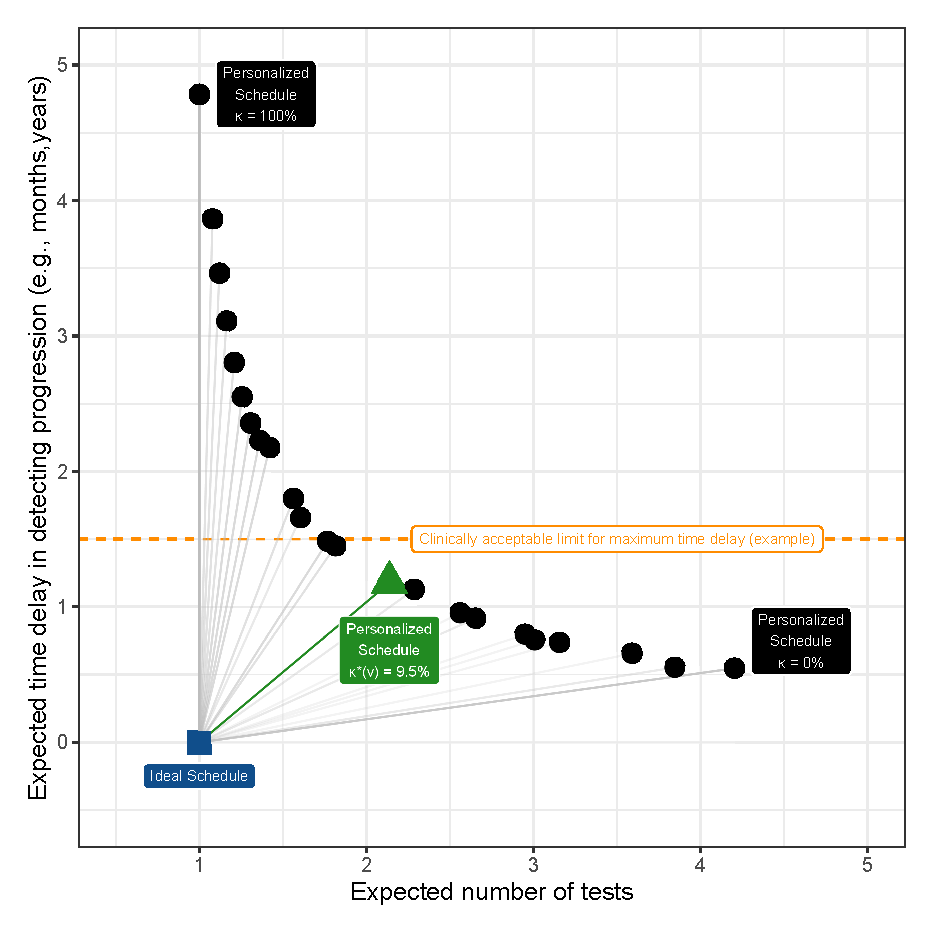
\includegraphics{images/kappa_choice_102.eps}}
\caption{\textbf{Automatic choice of risk threshold $0 \leq \kappa^* \leq 1$ using~(\ref{eq:kappa_choice})}. The ideal schedule of tests at point (1,0) is shown as a blue square. It plans exactly one invasive test at the true time of progression $T^*_j$ of a patient and hence leads to a zero time delay in detecting progression. Personalized schedules based on a grid of thresholds chosen between $0 \leq \kappa^* \leq 1$ are shown with black circles. Higher thresholds lead to fewer tests, but also higher expected time delay. We propose to choose the personalized schedule based on $\kappa^*(v)=19.5\%$ threshold (green triangle). This is because it has the least Euclidean distance (shown with a green line) to the ideal schedule. It is also possible to find the least distance under a certain clinically acceptable limit on time delay (orange dashed line), or number of tests.}
\label{fig:kappa_choice}
\end{figure}